73. В первом случае в пересечении образуется квадрат, раз его площадь равна $4\text{м}^2,$ его сторона равна 2м. Во втором случае образуется прямоугольник, горизонтальная сторона которого также равна 2м, а значит вертикальная сторона равна $14:2=7$м, она же является стороной меньшего ковра. Значит, сторона большего ковра равна $7\cdot2=14$м и сторона комнаты равна $12+2+5=19$м.
\begin{center}
\begin{figure}[ht!]
\center{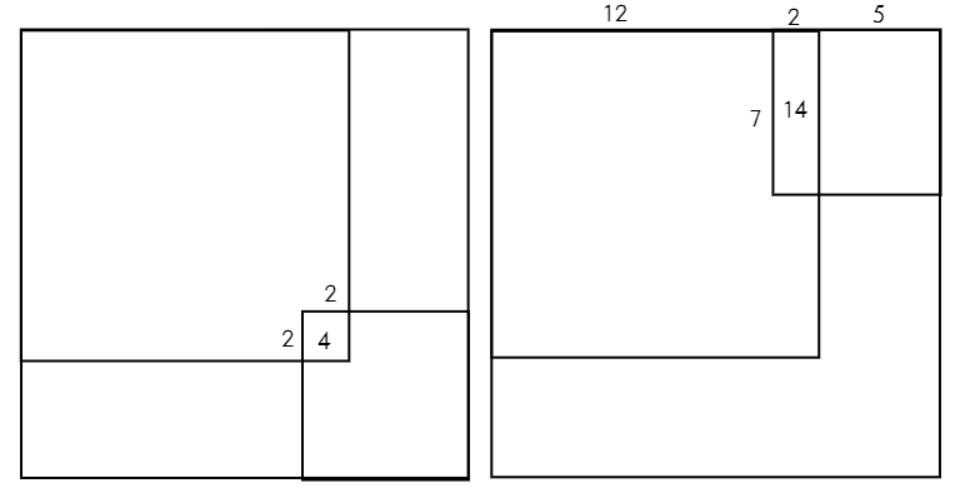
\includegraphics[scale=0.35]{sq.png}}
\end{figure}
\end{center}

ewpage

oindent74. В первом случае в пересечении образуется квадрат, раз его площадь равна $9\text{м}^2,$ его сторона равна 3м. Во втором случае образуется прямоугольник, горизонтальная сторона которого также равна 3м, а значит вертикальная сторона равна $15:3=5$м, она же является стороной меньшего ковра. Значит, сторона большего ковра равна $5\cdot2=10$м и сторона комнаты равна $7+3+2=12$м.
\begin{center}
\begin{figure}[ht!]
\center{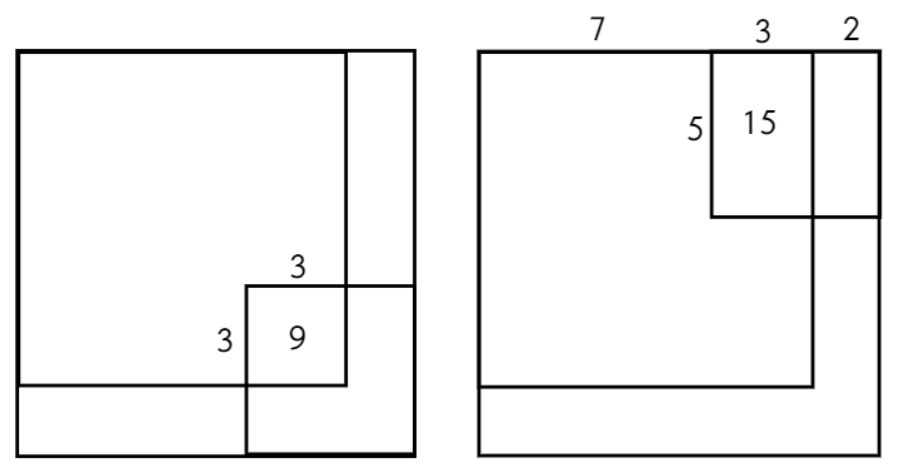
\includegraphics[scale=0.35]{sq1.png}}
\end{figure}
\end{center}
